\subsection{Data Collection and Preparation}
The Baby Connectome Project (BCP)\cite{howellUNCUMNBaby2019} is an accelerated longitudinal cohort acquired at the University of North Carolina at Chapel Hill (UNC) and the University of Minnesota (UMN) on 3T Siemens Prisma scanners. The dataset includes more than 1{,}000 structural (sMRI) and 400 diffusion (dMRI) scans from typically developing children imaged between birth and 5 years of age. Participants were recruited to approximate the demographic composition of the U.S. population, and written informed consent was obtained from parents or legal guardians under protocols approved by the UNC/UMN Institutional Review Boards. Harmonized acquisition protocols were implemented at both imaging sites, yielding no significant inter-site differences in image properties.

We also analyzed resting-state functional MRI (rs-fMRI) from the HBCD 1.0 release\cite{nelsonIntroductionHEALthyBrain2024}, comprising over 900 scans from 466 infants aged 0--6 months. Data were processed using our infant-centric pipeline, including motion correction, EPI distortion correction, boundary-based registration to T2-weighted images, and one-step resampling to native T2w space. Denoising was then performed using high-pass filtering and ICA-AROMA\cite{pruimICAAROMARobustICAbased2015}.

\noindent\underline{Structural MR images preprocessing.}
\hfill\\
T1-weighted (T1w) images were acquired on a \numproduct{320 x 320} matrix with a \numproduct{256 x 256}\,\unit{\milli\meter} field of view (FOV), 208 sagittal slices, and \SI{0.8}{\milli\meter} isotropic resolution (TE = \SI{2.24}{\milli\second}, TR = \SI{2400}{\milli\second}, flip angle = \SI{8}{\degree}). 
T2-weighted (T2w) images were acquired with a \numproduct{320 x 320} matrix, \numproduct{256 x 256}\,\unit{\milli\meter} FOV, 208 sagittal slices, and \SI{0.8}{\milli\meter} isotropic resolution (TE = \SI{564}{\milli\second}, TR = \SI{3200}{\milli\second}, variable flip angle). 
All images underwent standardized quality control and preprocessing\cite{liuMultistageImageQuality2019}, including intensity inhomogeneity correction, skull stripping, rigid T1w–T2w alignment, tissue segmentation, and cortical surface reconstruction (NeuroVerse pipeline)\cite{caliNeuroVerseImmersiveExploration2024}. 

\noindent\underline{Diffusion MR image preprocessing.}
Diffusion MRI data were acquired in pairs of scans with opposite phase-encoding directions (PEDs) using a 32-channel receiver coil, a \numproduct{140 x 140} imaging matrix, a \numproduct{210 x 210}\,\unit{\milli\meter} field of view (FOV), 95 axial slices, and \SI{1.5}{\milli\meter} isotropic resolution (TE = \SI{88}{\milli\second}, TR = \SI{2640}{\milli\second}, excitation flip angle = \SI{78}{\degree}, refocusing flip angle = \SI{160}{\degree}, multiband factor = 5, non-collinear gradient directions). 
For each PED, \num{9}, \num{12}, \num{17}, \num{24}, \num{34}, and \num{48} diffusion-weighted images (DWIs) were acquired at $b$-values of 500, 1000, 1500, 2000, 2500, and 3000\,\si{\second\per\milli\meter\squared}, respectively, together with 7 non-diffusion-weighted ($b = 0$\,\si{\second\per\milli\meter\squared}) volumes (one every 24 DWIs), yielding a total of 151 volumes for each of the posterior--anterior (PA) and anterior--posterior (AP) PEDs.

We processed the data using our baby-centric diffusion pipeline\cite{wu2021automated}. First, usable diffusion scans were identified with a deep-learning, semi-automated quality assessment (QA) algorithm\cite{liu2019multi}. After QA, 383 pairs of fMRI from 217 children (106 males, 111 females) were retained for further analysis; the age distribution of these scans is shown in Supplementary Fig.~\ref{fig:supplementary_population}. Next, we corrected for signal drop-out, pileup, and eddy-current- and susceptibility-induced distortions by leveraging rotation-invariant contrasts derived from diffusion spherical harmonic representations and structural MRI\cite{ahmad2020fast}. During this step, diffusion and structural images were co-registered using ANTs\cite{avants2009advanced}. All preprocessed scans underwent final visual inspection to ensure data quality, resulting in a total of 433 dMRI scans included in the study.

\noindent\underline{Functional MR images preprocessing}
Resting-state functional MRI data were acquired using a single-shot echo-planar imaging (EPI) sequence with 2\,mm isotropic resolution, a \SI{208}{\milli\meter} \(\times\) \SI{208}{\milli\meter} field of view, a \numproduct{104 x 104} acquisition matrix, TE = 37\,ms, TR = 800\,ms, flip angle = 52$^{\circ}$, and a total scan duration of 5\,min 47\,s.
Preprocessing was performed with FMRIB's Software Library (FSL, version 6.0\cite{smithAdvancesFunctionalStructural2004,jenkinsonFSL2012}) and comprised the following steps: 
\begin{inparaenum}[(i)]
    \item head motion correction using \texttt{mcflirt}\cite{jenkinsonImprovedOptimizationRobust2002}, which rigidly aligns each rs-fMRI frame to the single-band reference (SBref) image and outputs motion parameter estimates; 
    \item EPI distortion correction using \texttt{topup}\cite{anderssonHowCorrectSusceptibility2003,smithAdvancesFunctionalStructural2004}, with susceptibility-induced field inhomogeneities estimated from pairs of reversed phase-encoded fieldmaps; 
    \item rigid (6-DOF) registration of the SBref image to the fieldmap images; 
    \item rigid boundary-based registration (BBR)\cite{greveAccurateRobustBrain2009} of the distortion-corrected SBref to each subject’s T1-weighted anatomical scan, preceded by mutual-information-based pre-alignment; 
    \item one-step resampling in which all estimated deformation fields and linear transforms were concatenated and applied to the raw 4D rs-fMRI time series, yielding motion- and distortion-corrected volumes in native (T1w) space\cite{glasserMultimodalParcellationHuman2016}; 
    \item temporal high-pass filtering with a cutoff of 0.001\,Hz to remove low-frequency drifts; 
    \item attenuation of residual motion artifacts using ICA-based Automatic Removal Of Motion Artifacts (ICA-AROMA)\cite{pruimICAAROMARobustICAbased2015, parkesEvaluationEfficacyReliability2018}, implemented as a 150-component ICA with components classified as signal or noise based on spectral content, correlation with motion parameters, edge fraction, and CSF fraction, followed by non-aggressive regression of motion-related components; 
    \item nonlinear spatial normalization of the denoised data to Montreal Neurological Institute (MNI) space\cite{fonovUnbiasedNonlinearAverage2009,fonovUnbiasedAverageAgeappropriate2011}; 
    \item spatial smoothing with a 4\,mm FWHM Gaussian kernel in MNI space and intensity normalization to a global mean of 10{,}000\cite{glasserMinimalPreprocessingPipelines2013} to reduce scanner-related variability and enhance cross-subject comparability.
\end{inparaenum}

To ensure data quality, framewise displacement (FD) was computed from the motion parameters, and scans with mean FD (Power’s definition: sum of absolute parameter differences) greater than 0.5\,mm---a commonly used threshold in resting-state fMRI\cite{powerSpuriousSystematicCorrelations2012}---were excluded. In addition, skull stripping, tissue segmentation, and fMRI-to-T1w registration were visually inspected, and only datasets with acceptable quality were retained. After these procedures, 1{,}666 preprocessed rs-fMRI scans remained. From this pool, a subset with minimal motion and distortion was selected to construct the functional network template. In total, we analyzed 381 subjects with both fMRI and dMRI data.

\begin{figure}[t]
  \centering
  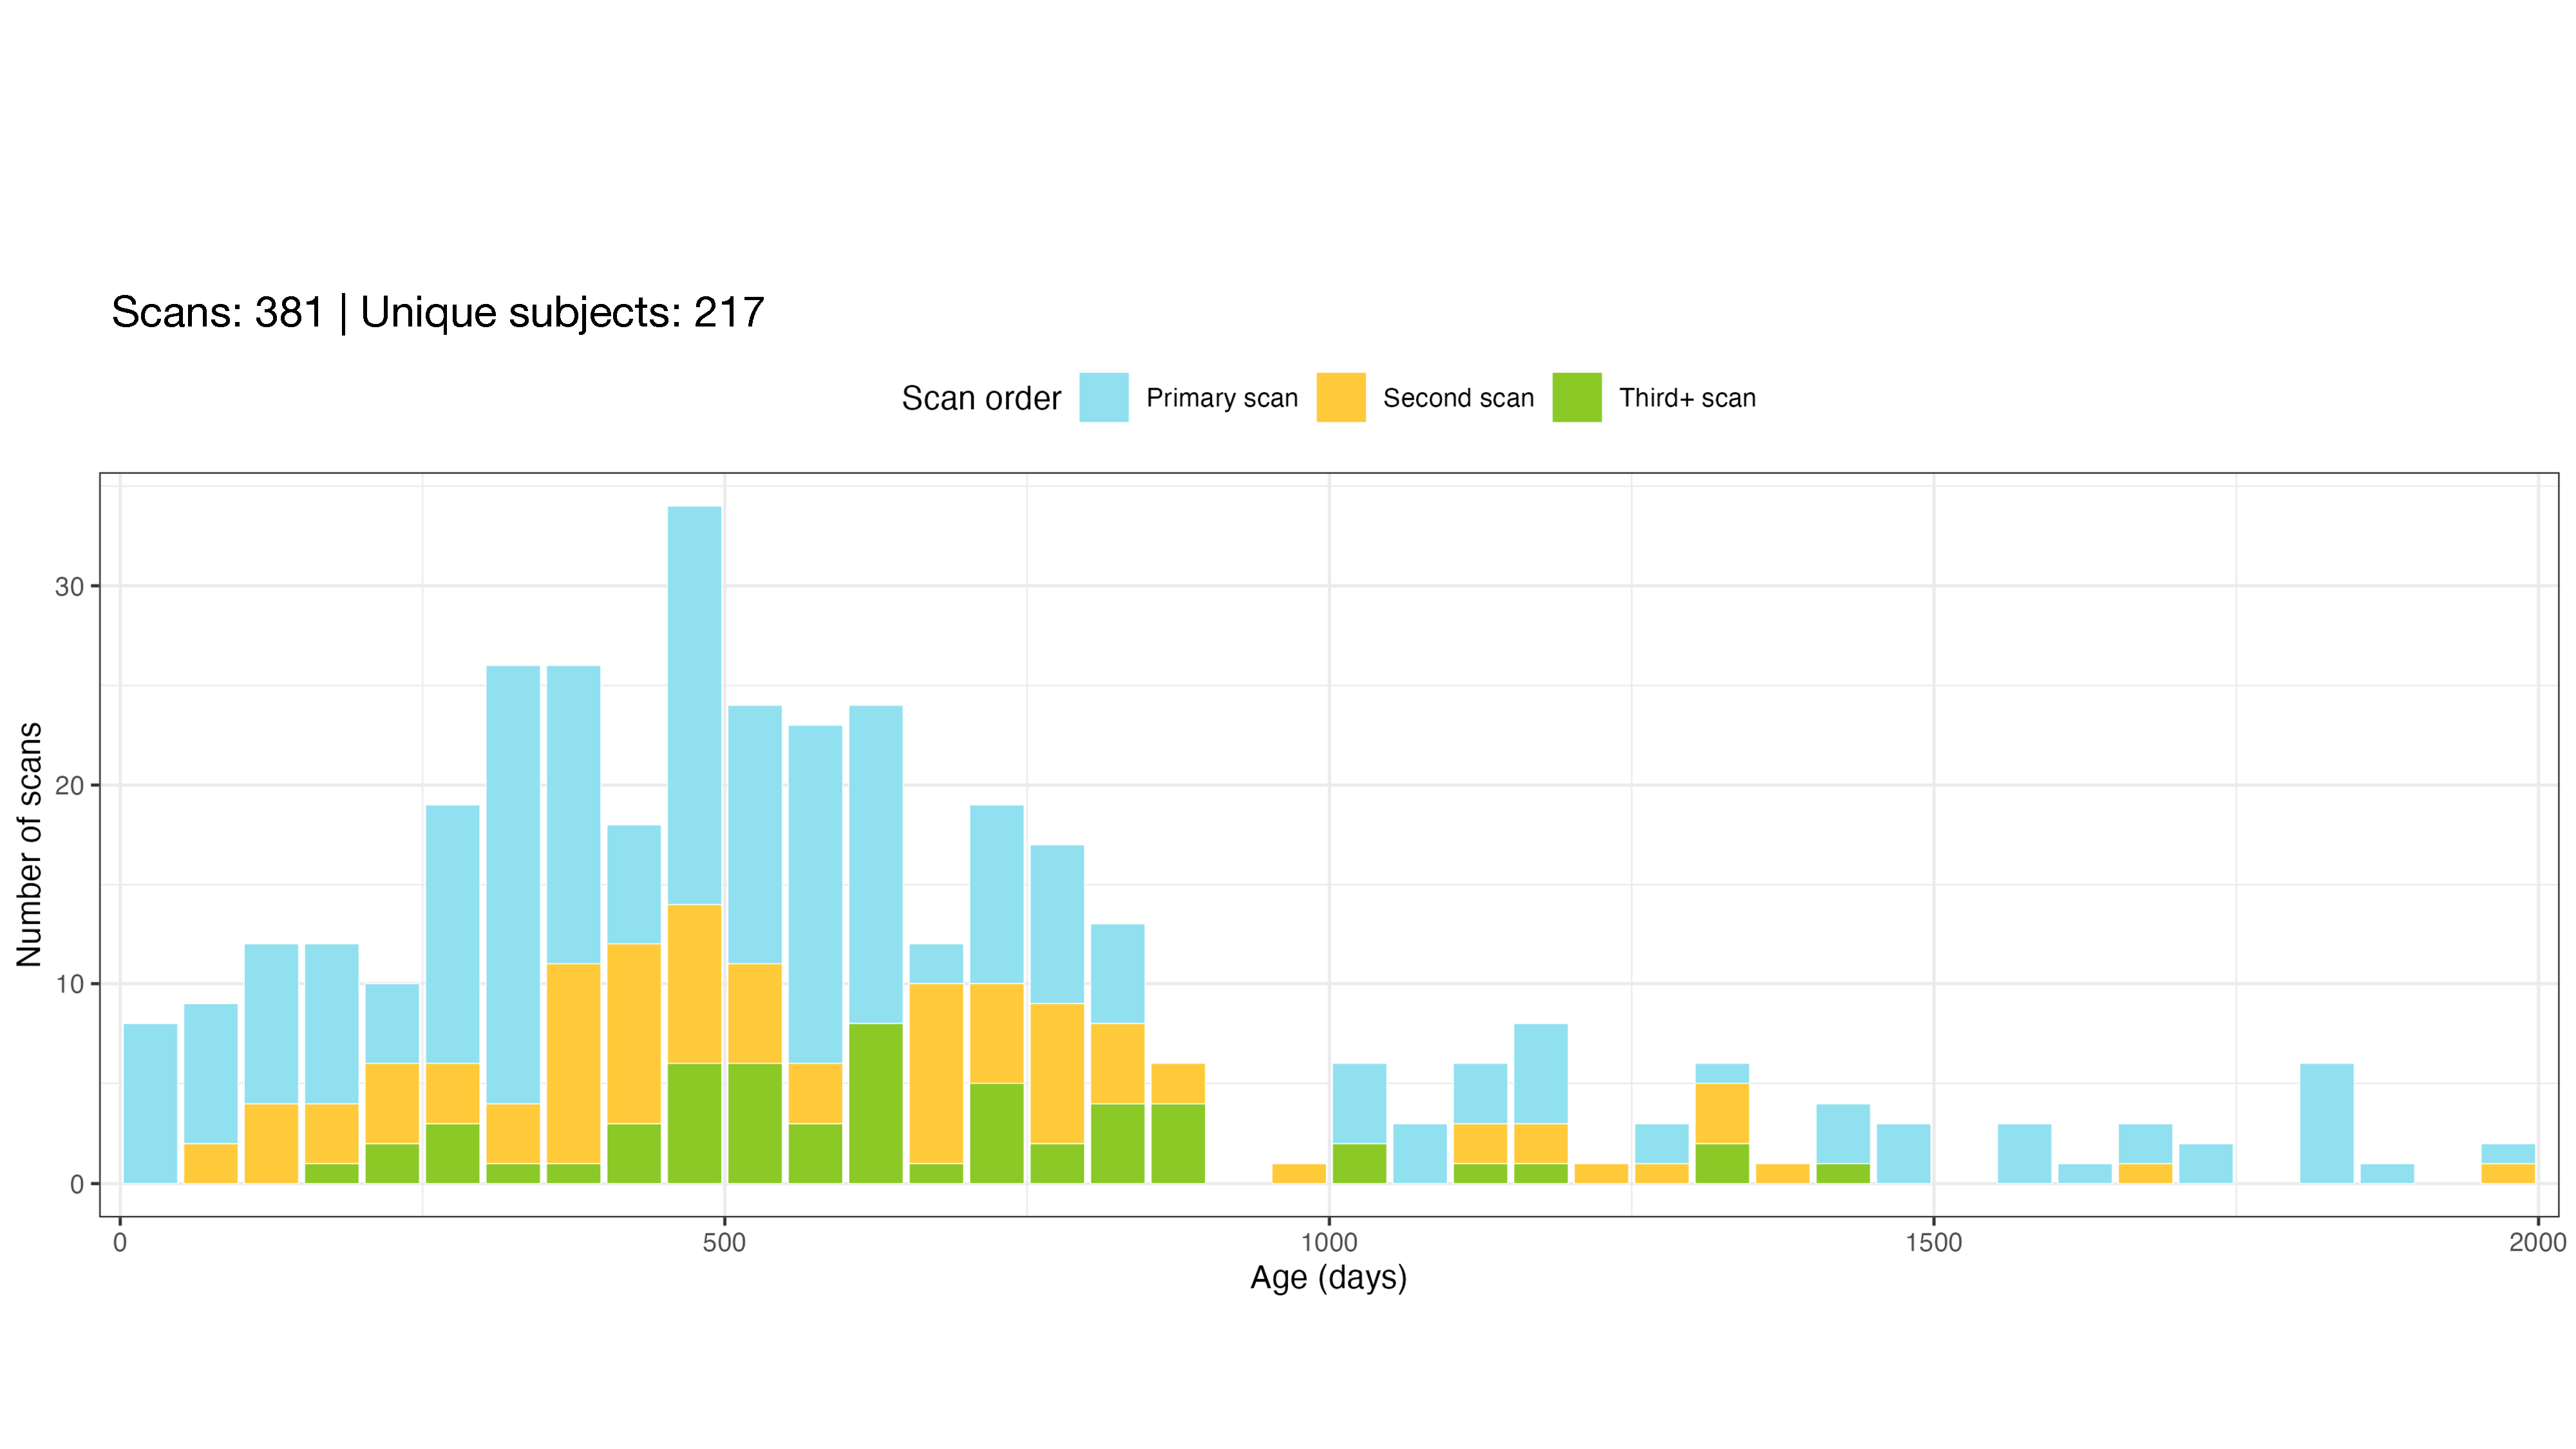
\includegraphics[width=0.95\linewidth]{figure/Figure1_population.pdf}
  \caption{\textbf{$|$ Population age distribution and sample composition.}
  Histogram bars show the distribution of matched scan ages (in days) across the early-childhood window analyzed in this study. Stacked colors indicate scan order within participant: first scan (blue), second scan (yellow), and third-or-later scan (green). We show three bin-width resolutions (20, 50, and 100 days) to illustrate both fine-grained and coarse-grained sampling density across age.}
  \label{fig:supplementary_population}
\end{figure}

\subsection{Denoising}\label{subsec:denoising}
Resting-state fMRI data from three healthy participants were obtained from the ON-Harmony dataset\cite{warringtonResourceDevelopmentComparison2023}. Data were acquired using a 3T Philips Achieva scanner with a repetition time of 1150\,ms (400 timepoints) and 2.4\,mm isotropic resolution. We compared our method, OS-SVD\cite{huynhOptimalShrinkageDenoising2024}, with two state-of-the-art techniques: MP-PCA\cite{veraartDiffusionMRINoise2016} and NORDIC\cite{vizioliLoweringThermalNoise2021}.
This denoising and individual-gradient evaluation framework follows our prior work on precision functional gradients and optimal-shrinkage fMRI denoising\cite{maoPrecisionFunctionalGradients2026,maoLoweringThermalNoise2024}.

\textbf{OS-SVD.} OS-SVD aggregates the time series of a group of neighboring voxels into a 2D matrix. It then applies singular value decomposition (SVD) followed by optimal shrinkage (OS) to separate signal and noise components.

\textbf{MP-PCA.} MP-PCA calculates the covariance matrix of the 2D signal matrix and uses Marcenko-Pastur (MP) curve-fitting to separate signal and noise components.

\textbf{NORDIC.} NORDIC uses MP-PCA as its core denoising algorithm, but incorporates g-factor information for performance improvement.

Denoising performance was assessed using temporal signal-to-noise ratio (tSNR) and residual maps. We compared these denoising methods directly under matched preprocessing settings.
\begin{figure}[t]
  \centering
  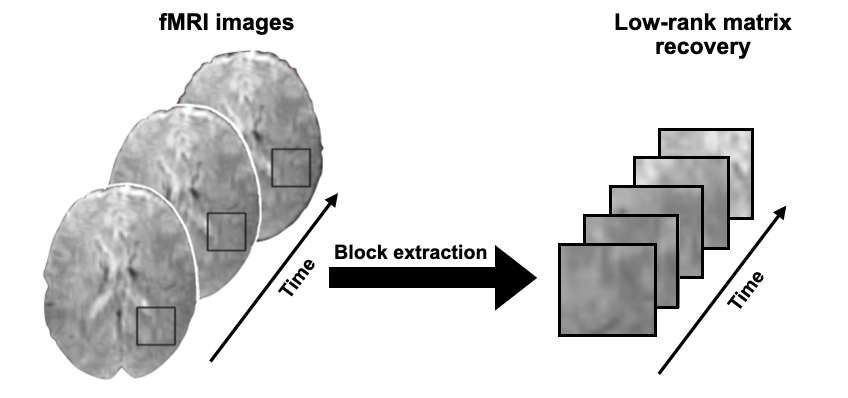
\includegraphics[width=0.95\linewidth]{figure/Figure2_denoising.png}
  \caption{\textbf{$|$ Denoising workflow.}}
  \label{fig:denoising_method}
\end{figure}

\subsection{Connectivity matrix construction}
\noindent\underline{Structural connectivity matrix}\label{subsec:SC} \hfill\\
% here there's an hdot between d1, d2 and dk is it supposed to be a value? 
Edge weights $A_{ij}$ connecting each pair of nodes in the adjacency matrix $A$ of each brain network were computed from the streamlines as follows. Each endpoint of a streamline can be associated with $K$ candidate vertices. Denoting the distances of the endpoint to the vertices as $0 \leq d_{1} \leq d_{2} \leq \hdots \leq d_{K}$, the connection weight for the $i$-th vertex can be defined as 
\begin{equation}
    w_{i} = \frac{\frac{1}{d_{i}}}{\sum_{k=1}^{K}\frac{1}{d_{k}}}.
\end{equation}
To avoid numerical complication when $d_{1} = 0$, we define $h_{i} = d_{1}/d_{i}$ with $h_{1} = 1$ and therefore
\begin{equation}
    w_{i} = \frac{h_{i}}{\sum_{k=1}^{K}h_{k}}.
\end{equation}
Considering two endpoints of a streamline, denoted with 1 and 2, the connection weight between vertices $i$ and $j$ is
\begin{equation}
    w_{ij} = w_{i}^{1}w_{j}^{2}.
\end{equation}
Note that $\sum_{i,j}w_{ij}=1$.
Streamlines causing self connections ($w_{ij}>0$ for $i=j$) are considered invalid and are excluded.
To account for regional size differences, streamline counts were normalized by the sum of the cortical volumes of the connected regions, yielding a matrix that reflects the relative strength of white matter connectivity between all region pairs. Finally, each subject's SC matrix was $z$-normalized. 

\noindent\underline{Functional connectivity matrix}\label{subsec:FC} \hfill\\
For each subject and scan, preprocessed resting-state fMRI data were projected onto the cortical surface, yielding vertex-wise time series for the left and right hemispheres (each \(10{,}242 \times 420\) vertices~\(\times\)~timepoints). Vertices containing zero or NaN values were excluded prior to analysis. Functional connectivity (FC) was computed within each temporal segment by calculating the Pearson correlation coefficient between the time series of all vertex pairs, resulting in a vertex-by-vertex correlation matrix. To enhance network specificity and reduce spurious connections, each vertex’s FC profile was sparsified by retaining only the strongest 10\% of correlations per row and setting the remaining values to zero. We then computed a profile-similarity kernel across vertices by treating each vertex's thresholded FC pattern as a feature vector and calculating pairwise cosine similarity between all vertices. The resulting similarity values were converted to a normalized angular kernel within the range \([0,1]\) according to  
\[
K = 1 - \frac{\arccos(\text{cosine similarity})}{\pi}.
\]
This kernel quantifies the degree of functional similarity between vertices, where higher values indicate more similar connectivity profiles. The resulting kernel matrices were inserted back into the full cortical surface space (left and right hemispheres combined; \(20{,}484 \times 20{,}484\)) and saved for subsequent analyses.

\subsection{Functional gradients}\label{subsec:functional_gradients}
Following the functional-gradient workflow described in prior work\cite{taylorFunctionalHierarchyHuman2024}, we computed subject-level cortical gradients from thresholded functional connectivity matrices. For each acquisition, vertex-wise FC was defined by Pearson correlation between BOLD time series:
\[
\mathrm{FC}_{ij}=\mathrm{corr}\!\left(x_i(t),x_j(t)\right), \quad i,j\in\{1,\dots,20484\}.
\]
For each subject, FC matrices were averaged across acquisitions, then row-wise sparsified by retaining the strongest 10\% of connections per row. We next computed profile similarity between thresholded FC profiles using cosine similarity and converted it to a normalized-angle affinity kernel:
\[
\cos_{ij}=\frac{f_i^\top f_j}{\|f_i\|\,\|f_j\|}, \qquad
K_{ij}=1-\frac{\arccos(\cos_{ij})}{\pi}, \quad K_{ij}\in[0,1],
\]
where \(f_i\) is the thresholded FC profile of vertex \(i\). Diffusion-map embedding (BrainSpace implementation) was applied to this affinity matrix. Let \(D\) be the degree matrix with \(D_{ii}=\sum_j K_{ij}\); the row-stochastic operator is
\[
P=D^{-1}K,
\]
and gradients were obtained from its leading non-trivial eigenvectors:
\[
P\psi_m=\lambda_m\psi_m, \qquad m=1,\dots,k.
\]
We extracted the first 10 gradients per subject and aligned them to a template gradient basis by one-shot orthogonal Procrustes (without scaling or mean-centering). Denoting subject and template gradients by \(X,Y\in\mathbb{R}^{N\times 10}\), we solved
\[
R^*=\arg\min_{R}\|XR-Y\|_F^2,\qquad \text{s.t. } R^\top R=I.
\]
Using \(M=X^\top Y=U\Sigma V^\top\), the optimal transform is
\[
R^*=UV^\top,\qquad X_{\text{aligned}}=XR^*.
\]
After alignment, each gradient sign was checked against the template and flipped when needed to preserve correspondence across subjects.

\begin{figure}[t]
  \centering
  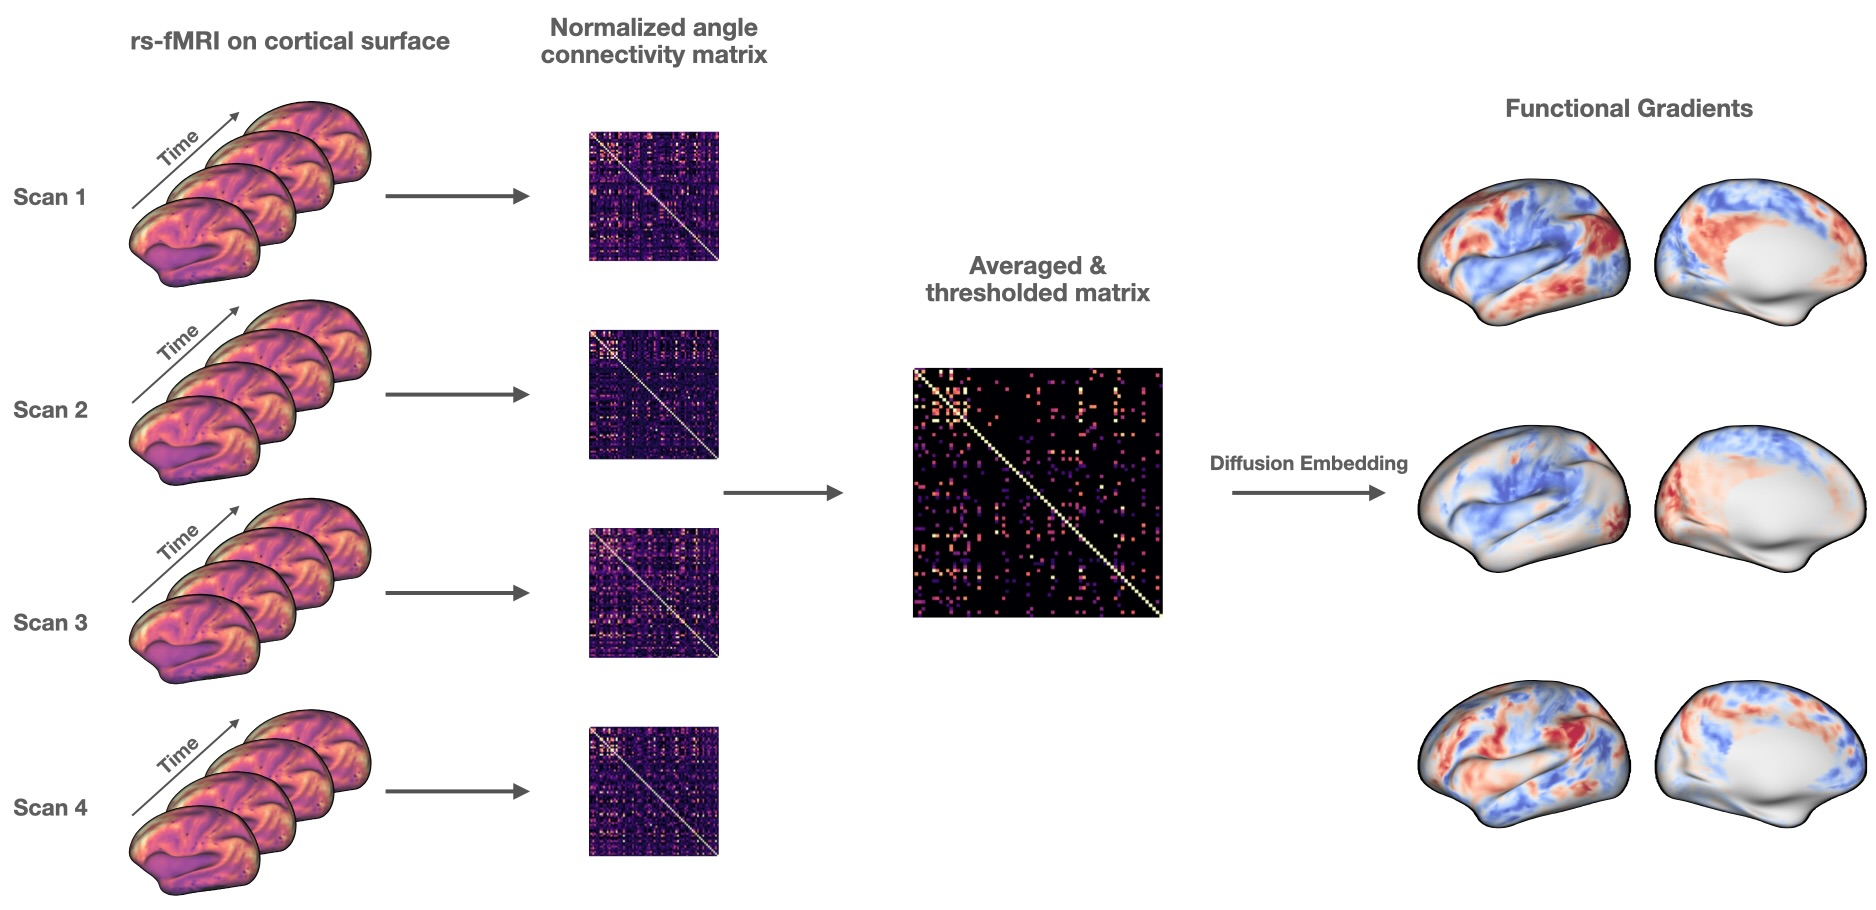
\includegraphics[width=0.95\linewidth]{figure/Figure3_individualgradients.jpeg}
  \caption{\textbf{$|$ Individual functional gradients and template alignment.}
  Subject-level cortical gradients were derived from thresholded FC profile similarity using diffusion-map embedding and aligned to the template basis using one-shot orthogonal Procrustes transformation.}
  \label{fig:individual_gradients}
\end{figure}

\clearpage
\subsection{Structure-Function Coupling (SFC)}\label{subsec:SFC}
SFC is calculated as the Pearson correlation between structural connectivity and functional connectivity profiles of each vertex. We calculated the Pearson correlation coefficient between these two profiles, resulting in a single SFC value for each vertex. This process was repeated for all vertices on the cortical surface, yielding a vertex-wise map of SFC for each subject. 
To quantify how much SFC fluctuates around its mean over time, we also computed a temporal SFC variance measure. 
Instead of estimating a single ``static'' SFC value per region, as in our primary analyses, we first divided each BCP scan (420 volumes) into 10 non-overlapping, temporally contiguous windows and computed a separate functional connectivity matrix for each window using the procedure described in the ``Functional Connectivity'' section. 
For each subject and each vertex, we then computed an SFC value within each window by relating that vertex's window-specific functional connectivity profile to its corresponding structural connectivity profile (excluding self-connections and entries in which either structural or functional connectivity was zero). 
This yielded 10 SFC values per vertex per subject. 
A vertex's temporal SFC variance was defined as the variance of these 10 time-resolved SFC estimates. 
Together with the static SFC metric (overall strength of structure--function coupling), this temporal SFC variance index captures how strongly a region's coupling to its structural backbone fluctuates over the course of the resting-state scan.

\begin{figure}[t]
  \centering
  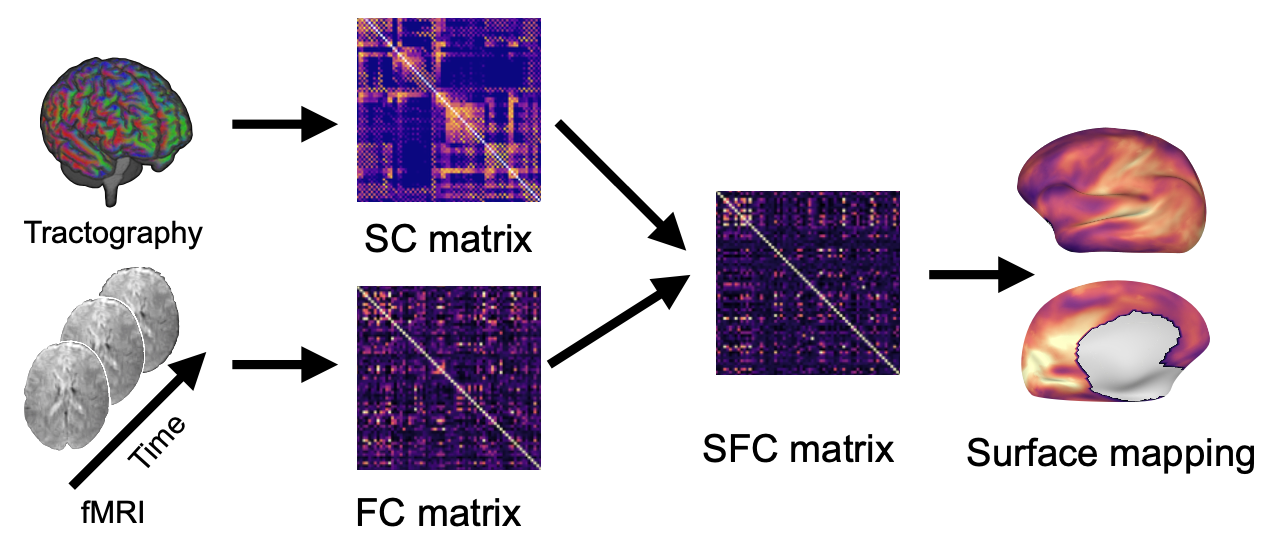
\includegraphics[width=0.95\linewidth]{figure/Figure4_SFCmethod.png}
  \caption{\textbf{$|$ Structure-function coupling (SFC) computation workflow.}
  Vertex-wise SFC was computed as the Pearson correlation between each vertex's structural and functional connectivity profiles, with additional time-windowed estimation used to derive temporal SFC variance.}
  \label{fig:sfc_method}
\end{figure}

\subsection{Excitation-inhibition balance}
Previous modeling work has shown that shifts in the excitation–inhibition ratio (E/I ratio) are reflected in the spectral properties of neural activity, in particular in the exponent of the 1/f power-law component, which is mathematically related to the Hurst exponent of the signal time series\cite{trakoshisIntrinsicExcitationinhibitionImbalance2020,bruiningMeasurementExcitationinhibitionRatio2020,gaoInferringSynapticExcitation2017}. This relationship has been validated both in simulated functional data and in mouse resting-state fMRI during chemogenetic modulation of pyramidal cell excitability, where an increased E/I ratio corresponds to a decrease in the Hurst exponent\cite{gaoInferringSynapticExcitation2017}.

We projected each subject's preprocessed resting-state fMRI data onto the cortical surface and obtained time series for 20,484 vertices (10,242 per hemisphere). The Hurst exponent was estimated from each vertex’s BOLD time series using a univariate maximum-likelihood framework in combination with a discrete wavelet transform. For each subject and vertex, we first estimated the power spectral density (PSD) by taking the median of the squared magnitude of the sliding-window short-time Fourier transform (STFT). We used the median rather than the mean (as in Welch's method) to better accommodate the non-Gaussian distribution of spectral estimates and to reduce the impact of extreme outliers\cite{gaoInferringSynapticExcitation2017}. To obtain the 1/f power-law exponent (log-log slope), we then fit a robust linear regression to the log-transformed PSD across the specified frequency band (30-50 Hz) and took the slope of this fit as the 1/f exponent\cite{gaoInferringSynapticExcitation2017}.

\begin{figure}[t]
  \centering
  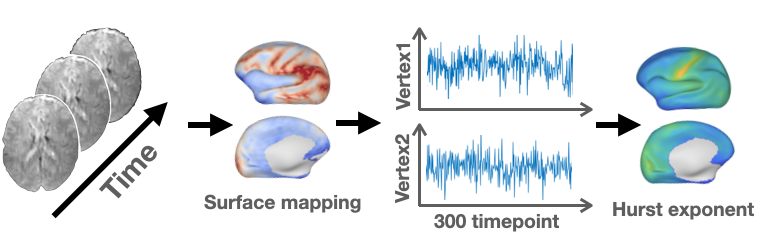
\includegraphics[width=0.95\linewidth]{figure/Figure5_hurstmethod.png}
  \caption{\textbf{$|$ Excitation-inhibition balance (Hurst) estimation workflow.}
  The Hurst exponent was estimated from vertex-wise rs-fMRI time series to index E/I-related dynamics across the cortex.}
  \label{fig:hurst_method}
\end{figure}

\subsection{Myelination calculation}\label{subsec:myeliation}
%i once have one sentence under fMRI preprocessing talk about it, can you pls check if this is true? 
Intracortical myelination was estimated using the T1w/T2w ratio, which has been shown to correlate with histological measures of myelin content\cite{glasserMappingHumanCortical2011}. For each subject, we computed the T1w/T2w ratio at each vertex on the cortical surface by dividing the intensity of the T1-weighted image by that of the T2-weighted image. This ratio was then normalized across subjects to account for inter-individual variability in signal intensity and to facilitate group-level analyses. The resulting vertex-wise myelin maps were used in subsequent analyses to examine their relationship with SFC and other developmental metrics.

\begin{figure}[t]
  \centering
  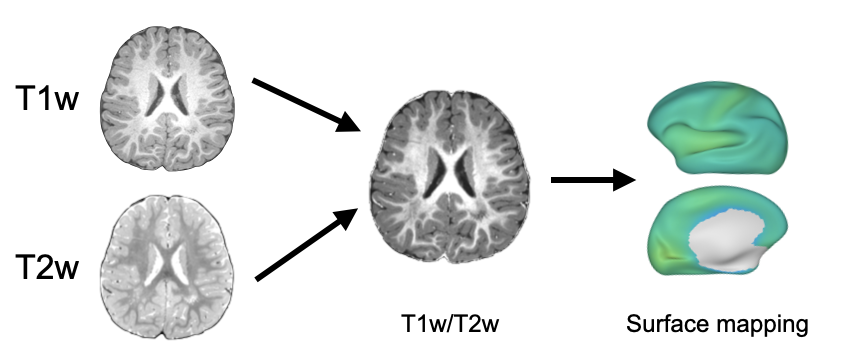
\includegraphics[width=0.95\linewidth]{figure/Figure6_myelinationmethod.png}
  \caption{\textbf{$|$ Intracortical myelination (T1w/T2w) computation workflow.}
  Vertex-wise T1w/T2w ratios were derived on the cortical surface to estimate intracortical myelin and used for downstream developmental analyses.}
  \label{fig:myelin_method}
\end{figure}

\subsection{Correlation calculation}\label{subsec:correlation}
\subsubsection{Spatial correlation}
For each timepoint $t$, we assembled two spatial maps across vertices: $X_t(v)$ (SFC) and $Y_t(v)$ (myelination or Hurst).  
We computed the Pearson correlation
\[
r_t = \mathrm{corr}\big(X_t(v), Y_t(v)\big)
\]
across $v = 1,\dots,10242$, with a two-sided p-value.  
This produced 401 spatial correlations per pairing (SFC-myelination and SFC-Hurst).  
Timepoints with $p < 0.001$ were considered significant. See more in \nameref{subsec:GAMM}.

\subsubsection{Temporal correlation}
For each subject-age timepoint (401 total), we derived vertex-wise maps on the fsaverage surface (10,242 vertices) for: (i) structure–function coupling (SFC), (ii) intracortical myelination (T1w/T2w ratio), and (iii) the Hurst exponent (functional time-series scaling).
For each vertex $v \in \{1,\dots,10242\}$, we formed two developmental trajectories across timepoints $t = 1,\dots,401$:  
$X_v(t)$ (SFC) and $Y_v(t)$ (either myelination or Hurst).  
We computed the Pearson correlation
\[
r_v = \mathrm{corr}\big(X_v(t), Y_v(t)\big)
\]
and its two-sided p-value. Vertices were considered significant at $p < 0.001$.  
This procedure was performed twice: (1) SFC–myelination and (2) SFC-Hurst, yielding two vertex-wise correlation maps.

\subsubsection{p-spin analysis}
To account for spatial autocorrelation on the cortical surface, we additionally performed a permutation spin test (p-spin) for each spatial-correlation analysis. In this framework, \(X\) was fixed as the vertex-wise SFC map and \(Y\) was the vertex-wise myelination map or Hurst map. We generated 1,000 spherical rotations of \(Y\) (within hemisphere), recomputed the correlation after each rotation, and built a null distribution \(\{r_t^{\mathrm{spin}}\}\). Two-sided spin-based significance was computed as
\[
p_{\mathrm{spin}}=\frac{1+\sum_{b=1}^{B}\mathbf{1}\!\left(|r_{t,b}^{\mathrm{spin}}|\ge |r_t|\right)}{1+B},
\]
with \(B=1000\). We report \(r_t\) together with \(p_{\mathrm{spin}}\) for both pairings (\(X=\) SFC, \(Y=\) myelination or Hurst).

\subsubsection{Mediation analysis}\label{subsec:mediation_pathway}
To complement vertex-wise correlation analyses, we performed scan-level pathway analyses to test whether microstructural and dynamical pathways explained SFC variation. For each scan, we derived one summary value per modality: mean SFC, mean Hurst exponent, mean T1w/T2w myelin, mean FC, and mean SC. For SFC, Hurst, and myelin, we first computed hemisphere-specific means and then averaged left and right hemispheres. SC and FC were reconstructed from part-wise 400-ROI files and aggregated to one scan-level mean connectivity value per modality.  

To align modalities across acquisitions, we anchored matching on SFC scans and matched the nearest same-subject scan from each other modality within a 30-day tolerance. For myelin, age values were converted from months to days using $\mathrm{Age}_{\mathrm{days}} = \mathrm{Age}_{\mathrm{months}} \times 30.5$ prior to matching.  

All pathway models were fit as linear mixed-effects models with subject-specific random intercepts to account for repeated longitudinal observations:
\[
Y_{ij} = \beta_0 + \beta_1 X_{ij} + (1 \mid \mathrm{ID}_i) + \epsilon_{ij},
\]
where $X_{ij}$ is the pathway predictor for subject $i$ at scan $j$, and covariates were held fixed across path equations within each model.
Model fitting and mediation workflows were implemented in R using broadly useful utilities from the \texttt{bruceR} package \cite{bao2021bruceR}.

\textbf{Direct pathway model.}  
For instance, for myelin $\rightarrow$ SFC fit:
\[
\mathrm{SFC}_{ij} = \gamma_0 + bM_{ij} + (1 \mid \mathrm{ID}_i) + \eta_{ij},
\]
where $M_{ij}$ denotes intracortical myelin.

\textbf{Serial mediation models.}  
For myelin $\rightarrow$ SC $\rightarrow$ SFC, we fit:
\[
\mathrm{SC}_{ij} = \delta_0 + d_{21}M_{ij} + (1 \mid \mathrm{ID}_i) + \epsilon_{2,ij},
\]
\[
\mathrm{SFC}_{ij} = \gamma_0 + b_1M_{ij} + b_2\mathrm{SC}_{ij} + (1 \mid \mathrm{ID}_i) + \eta_{ij}.
\]
For this model, the serial indirect effect is:
\[
IE_{\mathrm{serial}} = d_{21}b_2.
\]
The direct and total effects of myelin on SFC are:
\[
b_{\mathrm{direct}} = b_1,\qquad
b_{\mathrm{total}} = b_1 + d_{21}b_2.
\]

\textbf{Age-dependent mediation extension.}
To allow pathway strengths to vary developmentally, we additionally expressed path
coefficients as age-dependent functions:
\[
\mathrm{SC} = d_{21}(t)M + \epsilon_2,\quad
\mathrm{SFC} = b_1(t)M + b_2(t)\mathrm{SC} + \epsilon_Y.
\]
Age-specific serial indirect effects were defined as:
\[
IE_{\mathrm{serial}}(t)=d_{21}(t)b_2(t).
\]
For summary, we report peak serial mediation magnitude and its timing:
\[
IE_{\max}=\max_t |IE_{\mathrm{serial}}(t)|,\qquad
t^*=\arg\max_t |IE_{\mathrm{serial}}(t)|.
\]
Because averaging age-specific indirect effects is a different estimand from the
age-independent serial indirect effect, we prioritize trajectory-level summaries over a
single global mean effect.

\textbf{Integrated dual-channel model.}  
We additionally fit a piecewise integrated model combining structural and dynamics channels:
myelin $\rightarrow$ SC $\rightarrow$ SFC and Hurst $\rightarrow$ FC $\rightarrow$ SFC, with direct myelin $\rightarrow$ SFC and Hurst $\rightarrow$ SFC paths in the final outcome equation. Channel-specific and total indirect effects were computed as products/sums of fitted path coefficients.

Uncertainty for direct and indirect effects was estimated using subject-level bootstrap resampling (2,000 replicates), with 95\% percentile confidence intervals. For indirect effects, two-sided bootstrap p-values were computed from the smaller tail proportion relative to zero. For models containing multiple indirect pathways (e.g., integrated dual-channel models), multiplicity across indirect effects was controlled at $\alpha_{\mathrm{FWER}}=0.05$ using Holm correction (Bonferroni shown as reference). We also tracked the number of bootstrap replicates showing singular mixed-model fits as a model-stability diagnostic.

\subsubsection{Generalized Additive Mixed Modeling}\label{subsec:GAMM}
We used Generalized Additive Mixed Model (GAMM) curve fitting to model nonlinear changes of each brain feature over a time window of 0 to 5 years. To capture rapid developmental changes in the early postnatal stage, we applied a log transformation to the age variable.
For each vertex, we modeled changes $y$ as a function of age $t$ (fixed effect), individual $s$ (random effect) to account for longitudinal scans. The model incorporated smooth nonlinear functions $s_{\cdot}$, intercept $\beta$, and error $\epsilon \in \mathcal{N}(0,\sigma^2)$: $y=f(t,s)=\beta + s_t(\log_2(t+1) + s_s(s) + \epsilon$ with $t$ in years.
We set $s_{\cdot}$ to be cubic regression splines and used restricted maximum likelihood (REML) for smoothing parameter estimation, following \cite{taylorFunctionalHierarchyHuman2024}.
The BCP dataset was acquired at two imaging sites: the University of North Carolina at Chapel Hill (UNC) and the University of Minnesota (UMN). However, we found no significant differences in data distribution, microstructural values, or cortical gradients between sites. Therefore, site effects were not included in our model. 

\noindent\underline{Age effect}
To assess the influence of age, we contrasted the explanatory power of a full model, which included a smooth term for log-transformed age, with that of a reduced model without age. 
We defined the age effect as the change in adjusted $R^2$ ($\Delta R_{\text{adj}}^2$) between the full and reduced models, such that $\Delta R_{\text{adj}}^2$ indexes the variance uniquely attributable to age\cite{luoTwoAxesWhite2026}.
